\subsection{Human Cognition}\label{subsec:human-brain-structure}

\subsubsection{Cells}

\begin{wrapfigure}[18]{r}{0.3\textwidth}
    \begin{center}
        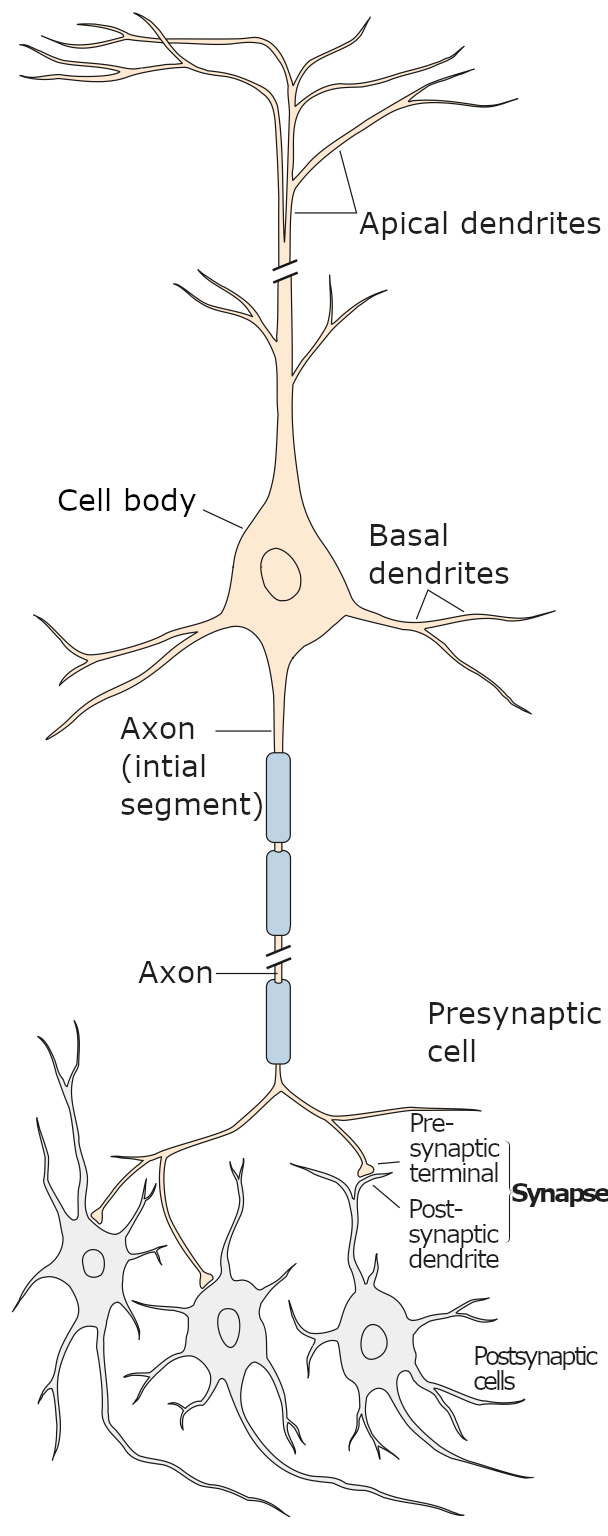
\includegraphics[width=0.28\textwidth]{images/neuron.jpeg}
    \end{center}
    \caption[Neuron]{The morphological structure of a neuron, taken from \citet[p. 22]{mack2013principles}}
    \label{fig:neuron_structure}
\end{wrapfigure}

The human nervous systems has two types of cells, \textit{neurons} and \textit{glial cells} or \textit{glia}~\citep[p. 71]{mack2013principles}.
Even though glia occur two to ten times more often in the nervous system than neurons~\citep[p. 24]{mack2013principles}, they - unlike neurons - \say{are not directly involved in electrical signaling}~\citep[p. 26]{mack2013principles} and therefore not further described in the course of this work.

Neurons in different brain regions can take different forms.
However, regardless of their specific configuration, they have four defined regions: \say{(1) the cell body, (2) dendrites, (3) axon, and (4) presynaptic terminals}~\citep[p. 22]{mack2013principles} (see Figure~\ref{fig:neuron_structure}).
The dendrites receive input from other neurons while axons convey electrical signals to other neuron's dendrites.
\textbf{Hier könnte noch deutlich mehr kommen.}

\subsubsection{Human Brain Structure}

The human brain is subdivided into six regions of different forms and functions: the medulla, pons, midbrain, cerebellum, diencephalon, and the cerebral hemispheres~\citep[p. 340]{mack2013principles} (see Figure~\ref{fig:human_brain_divisions}).
Together with the spinal cord, it constitutes the \ac{CNS}~\citep[p. 340]{mack2013principles}.

\begin{figure}
    \centering
    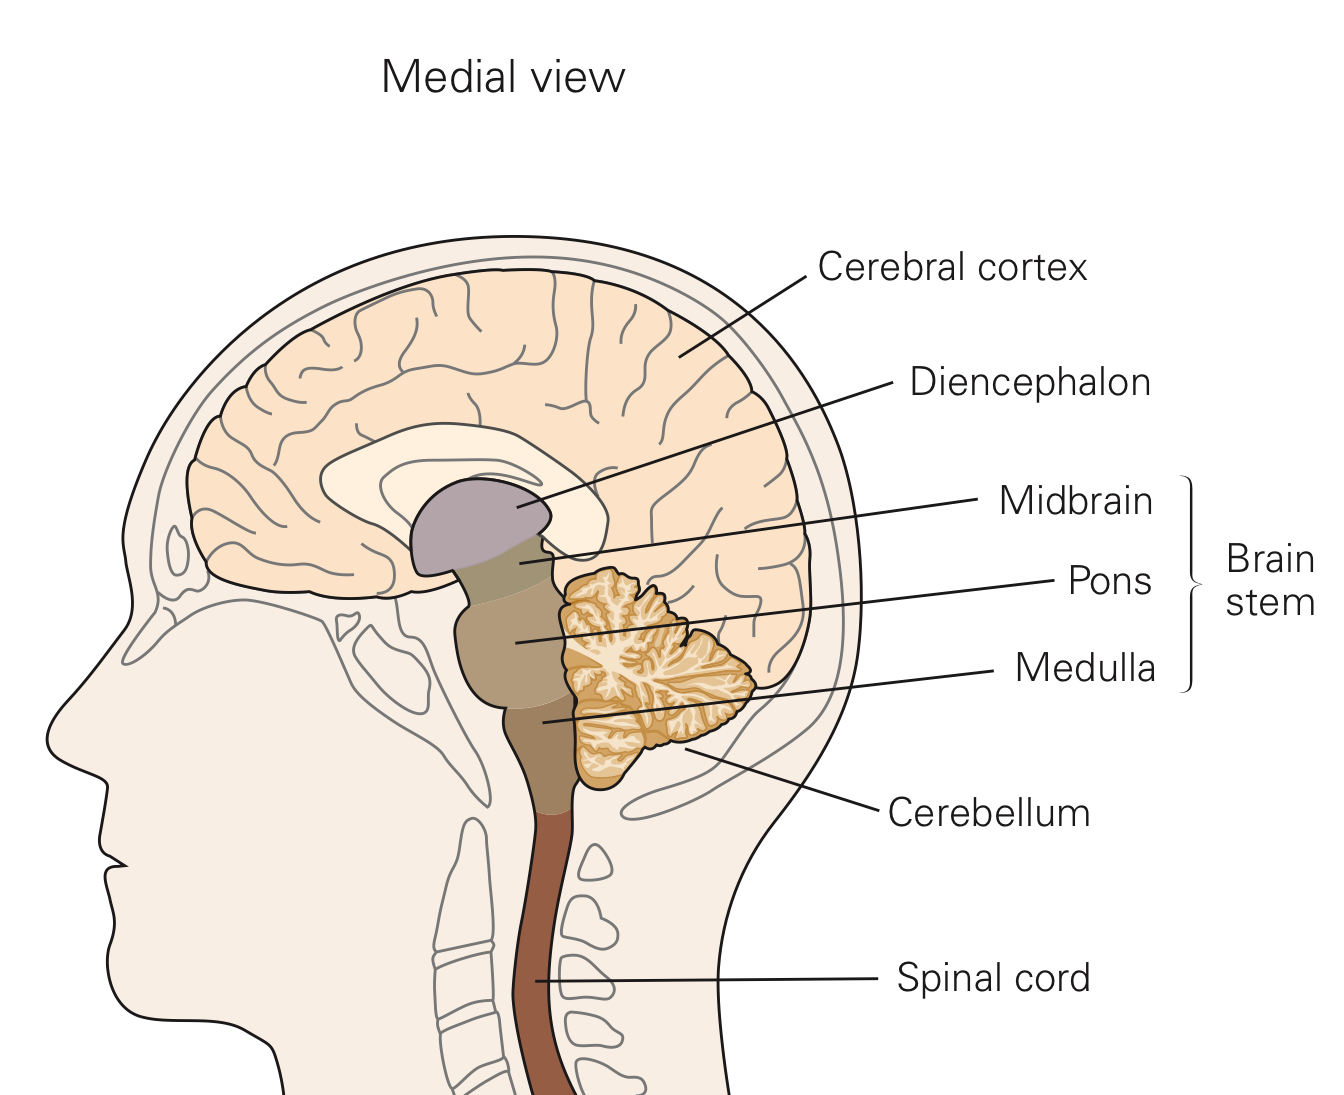
\includegraphics[width=.4\textwidth]{images/brain_regions.jpeg}
    \caption{Five divisions of the human brain, the cerebral cortex as part of the cerebral hemispheres, and the spinal cord. Taken from \citet[p. 340]{mack2013principles}.}
    \label{fig:human_brain_divisions}
\end{figure}

Medulla, pons, and midbrain constitute the \textit{brain stem}.
The brain stem recieves input from \say{several specialized senses, such as hearing, balance and taste} and \say{mediates sensation and motor control of head, neck, and face}~\citep[p. 341]{mack2013principles}.
Furthermore, it \say{contains [\ldots] pathways that carry [\ldots] information to other divisions of the \ac{CNS}}~\citep[p. 341]{mack2013principles}.

The \textit{cerebellum} is mostly responsible for motor skills but is also involved in \say{language and other cognitive function}~\citep[p. 341]{mack2013principles}.
Even though containing more neurons than other divisions of the brain, it \say{is well understood because relatively few types of neurons are involved}~\citep[p. 341]{mack2013principles}.

The \textit{diencephalon} contains the \textit{thalamus} and \textit{hypothalamus}.
The thalamus acts as a filter, deciding which information is forwarded to the neocortex~\citep[p. 341]{mack2013principles}.
The hypothalamus plays an important role in controlling body functions such as eating or drinking, but also in initiating behaviors~\citep[p. 341]{mack2013principles}.

The \textit{cerebral hemispheres}~\citep[p. 341]{mack2013principles}, finally, is the brain region most relevant for this thesis.
It can be further subdivided into \textit{cerebral cortex}, \textit{white matter}, \textit{basal ganglia}, \textit{amygdala}, and \textit{hippocampus}~\citep[p. 341]{mack2013principles}.
The latter three are \say{concerned with the expression of emotion [amygdala], [\ldots] memory formation [hippocampus], and [\ldots] control of movement and aspects of motor learning [basal ganglia]}~\citep[p. 342]{mack2013principles}.
The \textit{cerebral cortex}, underlayed by the \textit{white matter}, is the structure of the brain closest to the surface~\citet[p. 341]{mack2013principles}.

The \textit{neocortex} is \say{the region of cerebral cortex nearest the surface of the brain} \citet[p. 345]{mack2013principles}.
It is structured into six layers and columns~\citep[p. 345]{mack2013principles}.
Neurons within a column are assumed to from a \say{local processing network} and are understood as \say{the fundamental computational modules of the neocortex}~\citep[p. 348]{mack2013principles}.
Neurons within the different layers show different kinds of connectivity.
For example, Layer I mainly contains dendrites of cells in deeper layers where as Layers II and III contain \textit{pyramidal neurons} whose axons project onto other neuros~\citep[p. 346]{mack2013principles}.

Furthermore, the neocortex is structured \textit{topographically}, i.e.~neurons within a sensory area (e.g. the skin or retina) are mapped onto the neocortex such that neighboring neurons in the sensory area ultimately map onto neighboring regions in the neocortex~\citep[p. 343]{mack2013principles}.

\subsubsection{Visual Cortex}\label{subsubsec:visual-cortex}

The first cortical region receiving retinal signals is the \acf{V1}~\citep[p. 559]{mack2013principles}.
The \ac{V1} does not receive input directly from the retina, but the signal travels through the \textit{primary visual pathway} that includes the \ac{LGN}~\citep[p. 559]{mack2013principles}.
Two other pathways transport signals from the retina to other brain regions but are not concerned with object recognition but controlling movements and pupillary reflexes~\citep[p. 559]{mack2013principles}.

The \ac{LGN} contains so-called \textit{on-center} and \textit{off-center} cells that respond strongly to stimuli having either a bright center and a dark surrounding or a dark center and a bright surrounding~\citep[pp. 564-566]{mack2013principles}.
Noteworthy, the \ac{LGN} receives strong feedback from \ac{V1}.
However, the function of these feedback connections, outnumbering the number of feedforward neurons from the \ac{LGN} by the factor ten, \say{is largely unknown}~\citep[p. 573]{mack2013principles}.

\begin{figure}
    \centering
    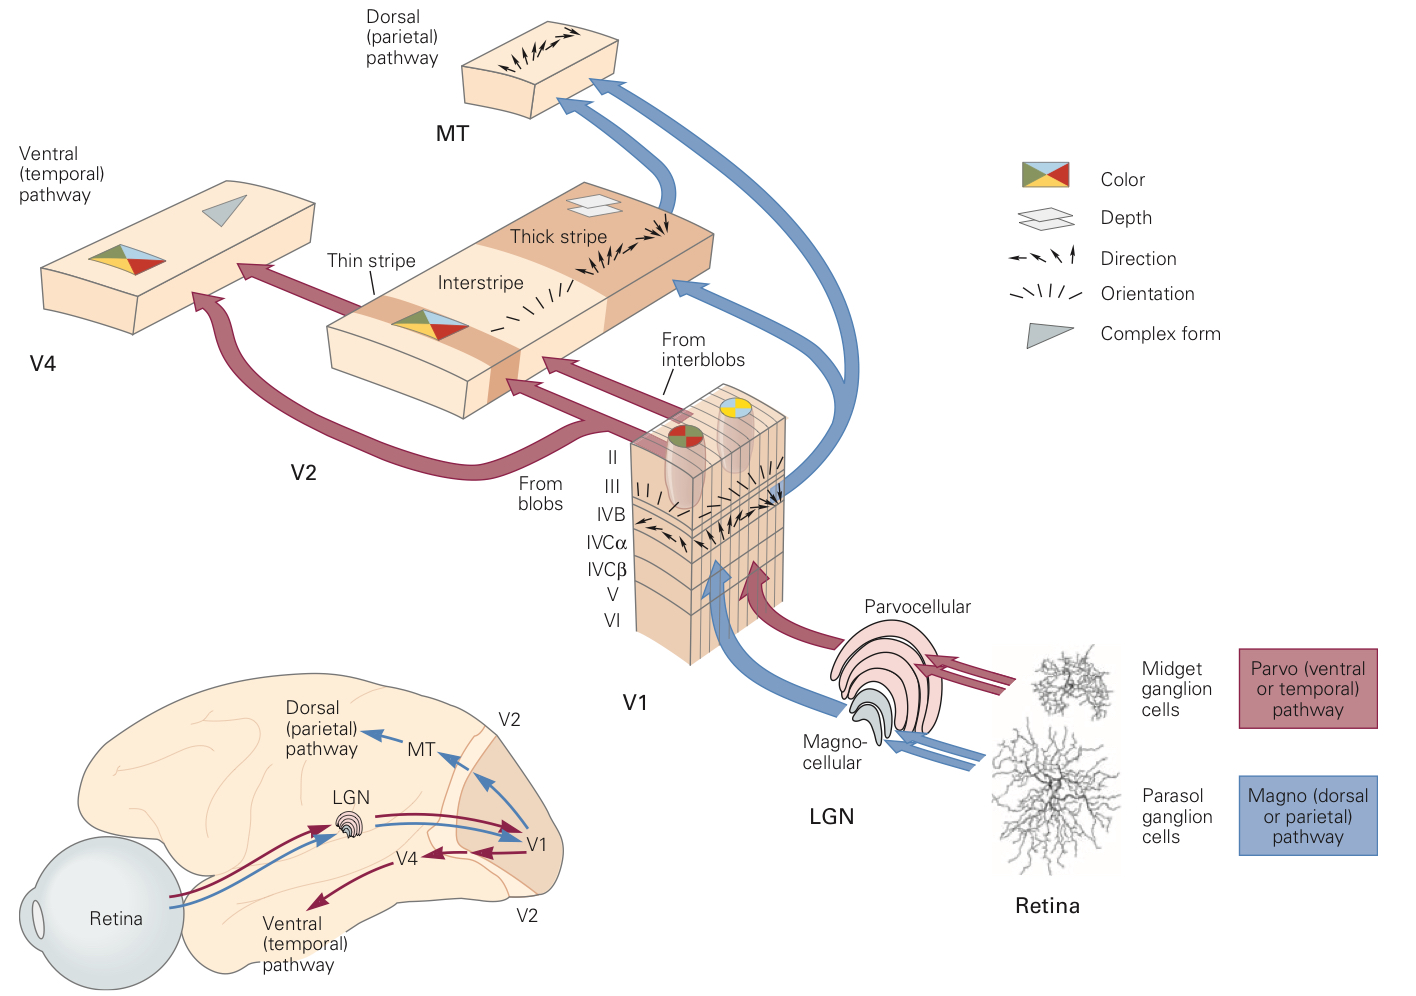
\includegraphics[width=.8\textwidth]{images/ventral_dorsal.jpeg}
    \caption{The ventral and dorsal pathways, carrying information from \ac{V1} to other brain regions. Taken from \citet[p. 571]{mack2013principles}}
    \label{fig:ventral_dorsal_pathway}
\end{figure}

From \ac{V1}, information is propagated to other brain regions via the \textit{ventral} and \textit{dorsal} pathways~\citep[pp. 563, 563]{mack2013principles}.
The dorsal pathway is responsible for the pass of information regarding the direction of movements whereas the ventral pathway is more concerned with object recognition~\citep[p. 564]{mack2013principles}.
Figure~\ref{fig:ventral_dorsal_pathway} shows the two pathways and the flow of information.
Importantly, Figure~\ref{fig:ventral_dorsal_pathway} does not show the complete pathways.
From V4, the Ventral pathways has feedback and feedforward connections from and to \ac{TEO}, and from \ac{TEO} it has feedback and feedforward connections from and to \ac{IT}, which, in turn, has feedback connections to \ac{V1} \citep[p. 563]{mack2013principles}.

According to the two-stream hypothesis~\citep{goodale1992separate}, the two pathways are assumed to encode the \textit{what} (dorsal) and \textit{where} (ventral) in a visual scene~\citep[p. 520]{mack2013principles}.
Even though the two pathways can exchange information \citep[p. 564]{mack2013principles}, they encode two different qualities of a stimulus: the identity and the location.

\subsection{Visual Object Perception}\label{subsec:visual-object-perception}

\begin{wrapfigure}[12]{r}{0.3\textwidth}
    \begin{center}
        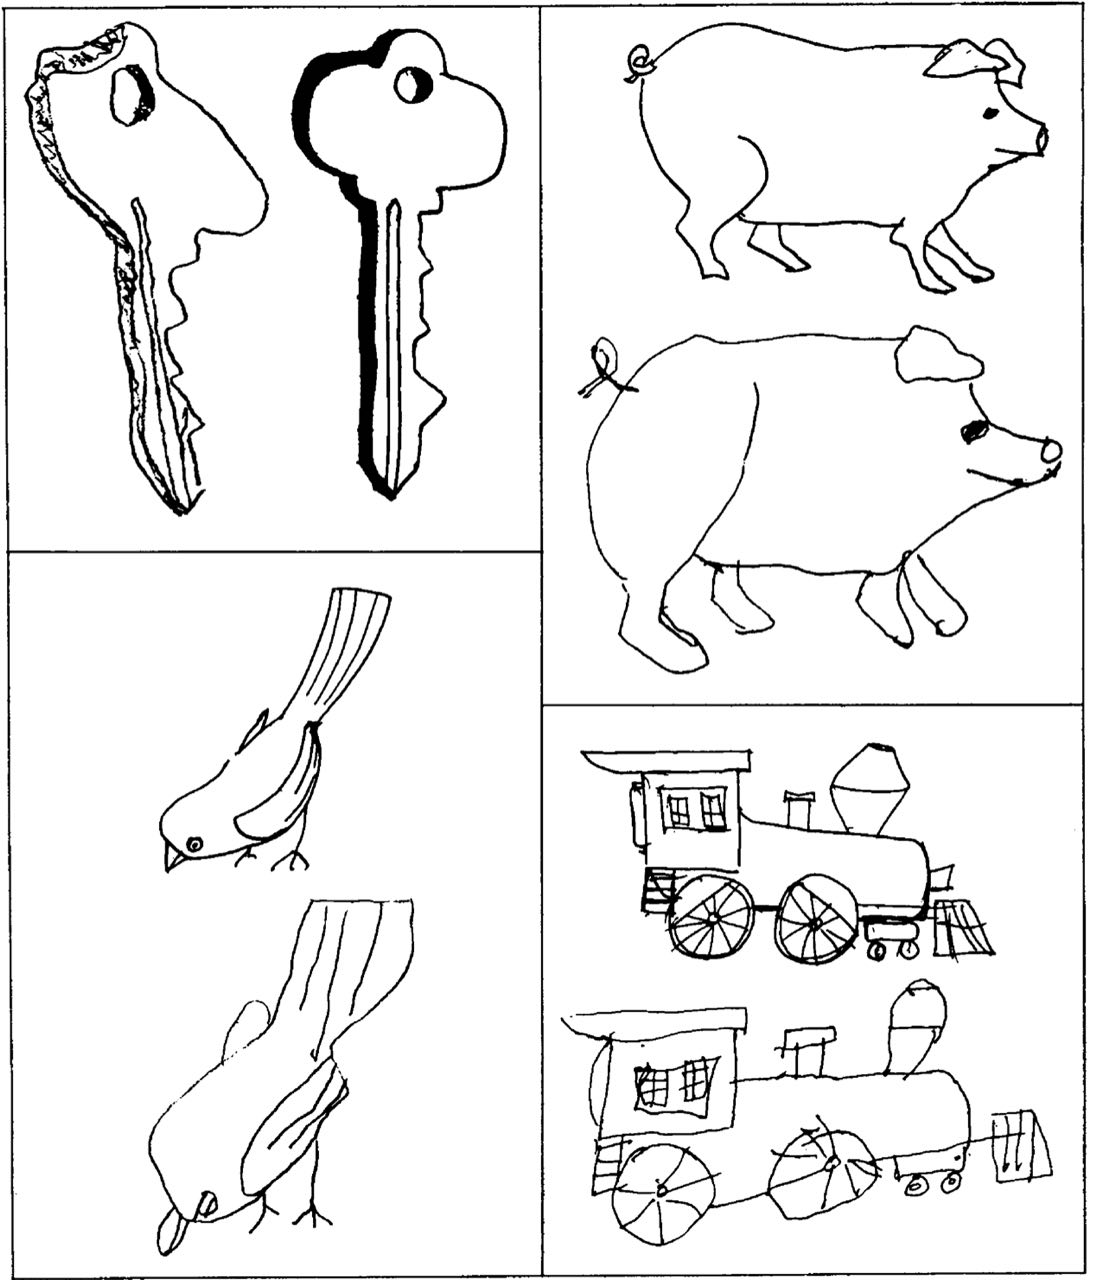
\includegraphics[width=0.28\textwidth]{images/rubens_sketches.jpg}
    \end{center}
    \caption[Copies of line drawings]{\say{Copies of line drawings.} taken from \citet{rubens1971associative}}
    \label{fig:copies_line_drawings}
\end{wrapfigure}
Recognizing an object as what it is is different from the ability of seeing an object or making a copy of it.
\citet{rubens1971associative} report the case of a 47-year old man who, on March 5--1969, \say{was found unconscious with vomitus on his face and bathrobe}.
Only after \say{his breathing became irregularly}, he was taken to a hospital where a low blood pressure was diagnosed.
The man showed an inability to recognize objects and in cases where he was unable to recognize an object, he also could not describe its use.
When given the category of an object, \say{identification improved very slightly}.
He claimed to recognize the item after being told the name.
In such cases, he was able to \say{point out various parts of the previously unrecognized item}.
When shown sketches of items, he was generally unable to recognize the items.
However, he was able to name geometric shapes such as circles or squares present in the sketch.
Even though the man did not recognize the objects, he was able to make copies of them (see Figure~\ref{fig:copies_line_drawings}).
\citet{rubens1971associative} report, that the Patient \say{was unable to identify any [items] before copying}.
However, he was able to contain some of the objects categories after copying them.

The example presented above shows that the ability to reproduce an object is different from the ability to \textit{perceive} it.

For monkeys, the \ac{IT} is assumed to be the brain region being crucial for object perception~\citep[pp. 1070, 1071]{squire2012fundamental}.
Bilateral lesions of the \ac{IT} in monkeys affect their ability to \say{distinguish between different visual patterns or objects, and in retaining previously acquired visual discriminations}~\citep[p. 1070]{squire2012fundamental}.
They are no longer able to generalize from tasks learned in one half of the visual space to the other half, presumably because the invariance of representations is lost~\citep[p. 1070]{squire2012fundamental}.
\citet[p. 1071]{squire2012fundamental} explicitly point out \say{the crucial role of the inferior temporal cortex during object perception and recognition}.

\subsection{Generative Methods}\label{subsec:generative-methods}

\subsubsection{\acfp{GAN}}

The idea behind \acp{GAN}~\citep{goodfellow2014gans} is to use two networks, one \textit{generator network} $G$ to approximate the data distribution, and one \textit{discriminator network} $D$ to discriminate between true data points and data points generated by the generator network.
This can be formalized as~\citep{goodfellow2014gans}:
\begin{align}
    \min _{G} \max _{D} V(D, G)=\mathbb{E}_{\bm{x} \sim p_{\text {data }}(\bm{x})}[\log D(\bm{x})]+\mathbb{E}_{\bm{z} \sim p_{\bm{z}}(\bm{z})}[\log (1-D(G(\bm{z})))] \label{eq:gan_objective}
\end{align}
where $\bm{z}$ is random noise.

The discriminator $D$ is trained towards predicting the correct label (\say{true datapoint}) for training samples $\bm{x}$ as well as for generated samples $G(\bm{z})$ (\say{fake samples}).
The generator $G$ is trained towards minimizing the probability that $D$ is capable of discriminating between true and fake samples.

\begin{figure}
    \centering
    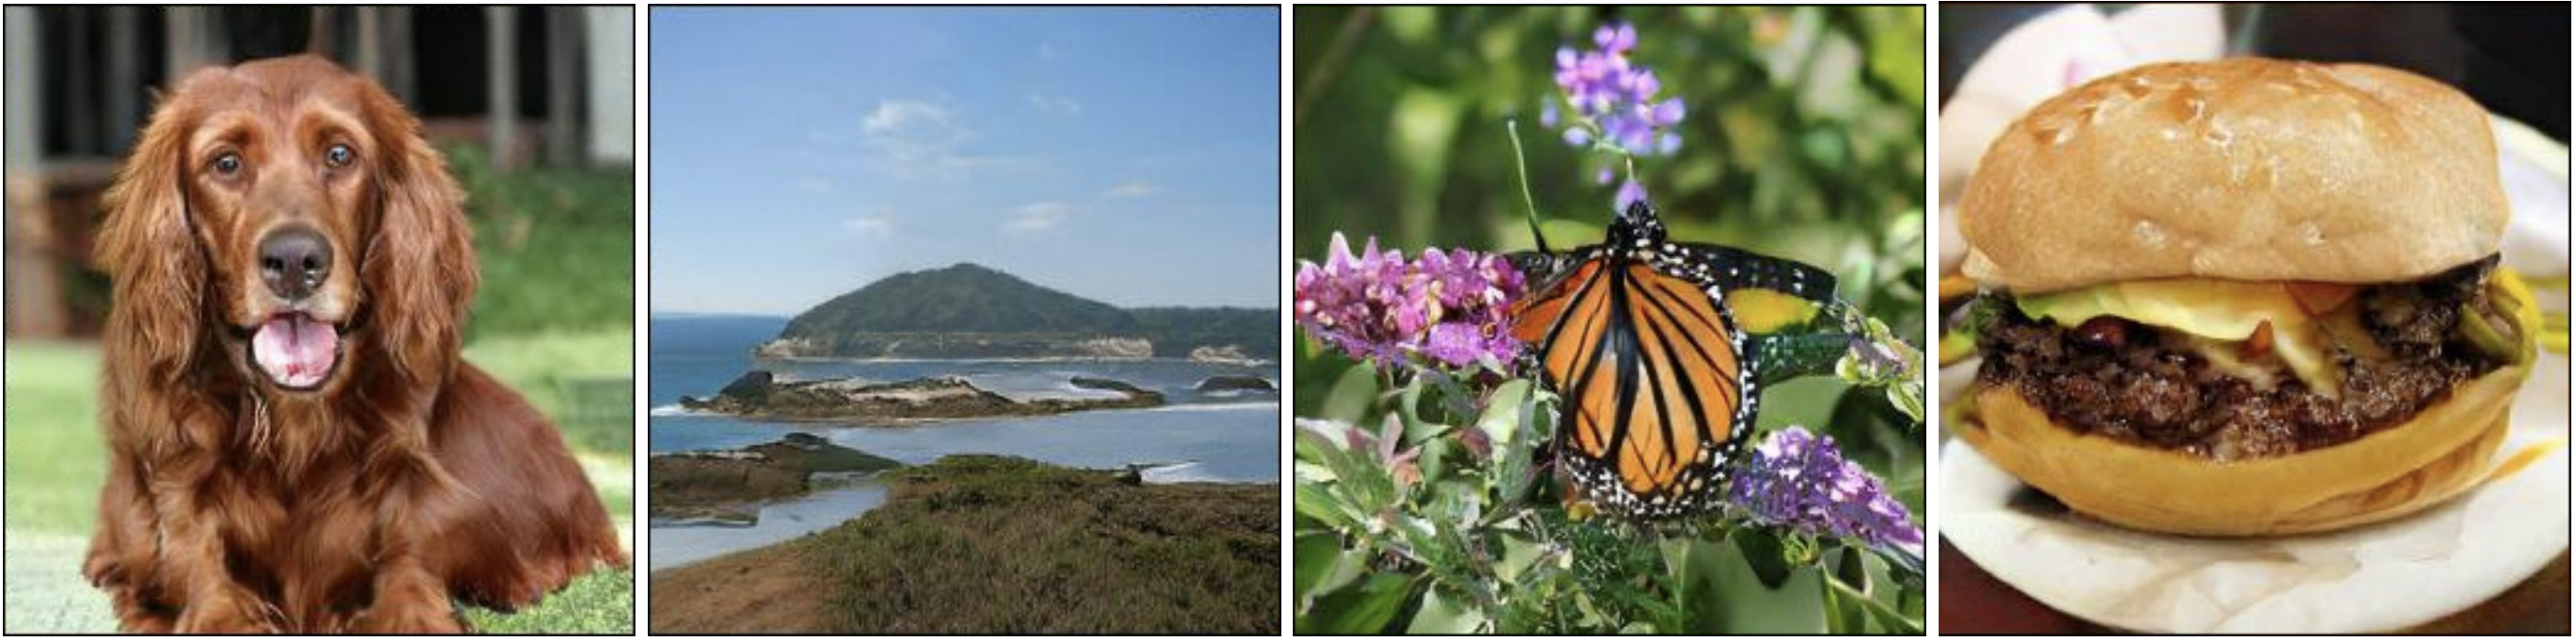
\includegraphics[width=\textwidth]{images/gan_samples.png}
    \caption{\ac{GAN}-generated samples, taken from \citet{brock2018large}.}
    \label{fig:gan_samples}
\end{figure}

Recent improvements on \acp{GAN} have led to synthesis of highly natural images as shown in Figure~\ref{fig:gan_samples}.

\subsubsection{Variational Autoencoders}\label{subsec:variational-autoencoders}

Since \acfp{VAE} are a specialization of the autoencoder, the traditional autoencoder is introduced first.

\paragraph{Autoencoders}

Autoencoders are neural networks trained to reconstruct their input~\citep[p. 499]{Goodfellow-et-al-2016}.
For autoencoders, it is common to speak of an \textit{encoder}-part and a \textit{decoder}-part.
The encoder $f: \mathbb{R}^n \mapsto \mathbb{R}^m$ transforms an input $\bm{x}$ to a hidden representation $\bm{r} = f(\bm{x})$.
Usually $m < n$, i.e.\ the encoder transforms the input to a lower-dimensional representation.
This can be beneficial for dimensionality reduction or feature learning~\citep[p. 499]{Goodfellow-et-al-2016}.
The decoder $g: \mathbb{R}^m \mapsto \mathbb{R}^n$ transforms the hidden representation back into the original feature space.
Usually, one wants the reconstruction $\tilde{x}$ to be close to the original feature $x$ ($\tilde{x} \approx x$).
In order to achieve this, the autoencoder is usually trained by minimizing $\mathcal{L}(\bm{x}, g(f(\bm{x})))$ with
\begin{align}
    \mathcal{L}: \mathbb{R}^n \times \mathbb{R}^n \mapsto \mathbb{R}
\end{align}
One common choice for $\mathcal{L}$ is the \ac{MSE} which is defined as
\begin{align}
    \mathcal{L}(\bm{x}, \bm{y}) = \frac{1}{n}\sum (\bm{x}_i - \bm{y}_i)^2 \label{eq:mse}
\end{align}~\citep[p. 106]{Goodfellow-et-al-2016}.
Note that for linear activations in the autoencoder, the space spanned by the first $m$ principal components is the optimal solution for equation~\ref{eq:mse}~\citep{chicco2014deep}.

\paragraph{Variational Autoencoders}

Autoencoders transform an input image to a \textit{hidden representation} $f(\bm{x})$.
However, the distribution over $f(\bm{x})$ is generally unknown.
Let $\bm{z} = f(\bm{x})$.
Assume $\bm{\tilde{z}} = \bm{z} + \bm{\epsilon}$ is a slightly perturbed version of $\bm{z}$, created by adding a small amount of noise $\bm{\epsilon}$.
Even though $\bm{\tilde{z}} \approx \bm{z}$, for example in terms of equation~\ref{eq:mse}, the result after decoding can be very different, i.e. $g(\bm{\tilde{z}}) \not\approx g(\bm{z})$ (again, in terms of equation~\ref{eq:mse}).
This is because the distribution $P(\bm{z})$ can take any arbitrary form.
Values of $\bm{z}$ that are one close to another\footnote{For example in terms of Euclidean distance} can be likely for very different values of $\bm{x}$.

To \textit{generate} new images it would be advantageous to enforce $P(\bm{z})$ to follow a certain distribution.
A common choice is a multivariate normal distribution without covariances~\citep[pp. 24, 25]{kingma2019introduction}.
\acp{VAE} enforce a certain (usually Gaussian) distribution over $\bm{z}$.

\acp{VAE} are trained to generate samples that are likely to occur in the training set.
Therefore, they aim to maximize $\log p(\bm{x})$\footnote{Please not that $\max \log  p(\bm{x}) \equiv \max  p(\bm{x})$.}~\citep[p. 18]{kingma2019introduction}.
Assuming a latent distribution $p(\bm{z})$ over $\bm{z}$, we can write $p(\bm{x})$ as the marginal distribution
\begin{align}
    p(\bm{x}) &= \int p(\bm{x}, \bm{z})d\bm{z} \label{eq:vae_x1}\\
    &= \int p(\bm{x}|\bm{z})\,p(\bm{z})d\bm{z} \label{eq:vae_x2}
\end{align}
Unfortunately, due to the integral w.r.t. $\bm{z}$ in equations~\ref{eq:vae_x1} and~\ref{eq:vae_x2}, computing $p(\bm{x})$ is intractable~\citep[p. 13]{kingma2019introduction}.
However, if the posterior $p(\bm{z}|\bm{x})$ was given, $p(\bm{x})$ could be obtained by
\begin{align}
    p(\bm{x}) = \frac{p(\bm{x}, \bm{z})}{p(\bm{z}|\bm{x})}
\end{align}
since computing $p(\bm{x}, \bm{z})$ is tractable~\citep[p. 14]{kingma2019introduction}.

\acp{VAE} approximate the posterior by an \textit{inference model} $q_\phi(\bm{z}|\bm{x}) \approx p_\theta(\bm{z}|\bm{x})$, also called the \textit{encoder}~\citep[p. 15]{kingma2019introduction}.

To make $q$ to match $p$ closely, usually the \ac{KL-divergence} plus the reconstruction error is minimized.
The reason for this is explained in the following.
The starting point is that we cannot compute the posterior $p_\theta(\bm{z}|\bm{x})$.
Therefore, we approximate it by another distribution $q_\phi$.
To make these two as similar as possible we use the \ac{KL-divergence} $\kldiv{q_\phi(\bm{z}|\bm{x})}{p_\theta(\bm{z}|\bm{x})}$

\begin{align}
    \kldiv{q_\phi(\bm{z}|\bm{x})}{p_\theta(\bm{z}|\bm{x})} &= -\sum_{\bm{z}} q_\phi(\bm{z}|\bm{x}) \log \frac{p_\theta(\bm{z}|\bm{x})}{q_\phi(\bm{z}|\bm{x})} \\
    &= -\sum_{\bm{z}} q_\phi(\bm{z}|\bm{x}) \log \frac{\frac{p_\theta(\bm{x},\bm{z})}{p_\theta(\bm{x})}}{\frac{q_\phi(\bm{z}|\bm{x})}{1}}\\
    &= -\sum_{\bm{z}} q_\phi(\bm{z}|\bm{x}) \log \frac{p_\theta(\bm{x},\bm{z})}{q_\phi(\bm{z}|\bm{x})}\frac{1}{p_\theta(\bm{x})}\\
    &= -\sum_{\bm{z}} q_\phi(\bm{z}|\bm{x}) \left[ \log \frac{p_\theta(\bm{x},\bm{z})}{q_\phi(\bm{z}|\bm{x})} - \log p_\theta(\bm{x}) \right]\\
    &= -\sum_{\bm{z}} q_\phi(\bm{z}|\bm{x}) \log \frac{p_\theta(\bm{x},\bm{z})}{q_\phi(\bm{z}|\bm{x})} + \sum_{\bm{z}} q_\phi(\bm{z}|\bm{x}) \log p_\theta(\bm{x}) \\
    &= -\sum_{\bm{z}} q_\phi(\bm{z}|\bm{x}) \log \frac{p_\theta(\bm{x},\bm{z})}{q_\phi(\bm{z}|\bm{x})} + \log p_\theta(\bm{x}) \underbrace{\sum_{\bm{z}} q_\phi(\bm{z}|\bm{x})}_{=1} \\
    &= -\sum_{\bm{z}} q_\phi(\bm{z}|\bm{x}) \log \frac{p_\theta(\bm{x},\bm{z})}{q_\phi(\bm{z}|\bm{x})} + \log p_\theta(\bm{x})
\end{align}
Then
\begin{align}
    \underbrace{\vphantom{\sum_{\bm{z}} x}\log p_\theta(\bm{x})}_{\text{constant}} =  \underbrace{\vphantom{\sum_{\bm{z}} x}\kldiv{q_\phi(\bm{z}|\bm{x})}{p_\theta(\bm{z}|\bm{x})}}_{\downarrow}  + \underbrace{\sum_{\bm{z}} q_\phi(\bm{z}|\bm{x}) \log \frac{p_\theta(\bm{x},\bm{z})}{q_\phi(\bm{z}|\bm{x})}}_{\uparrow}
\end{align}
Now, because $\log p_\theta(\bm{x})$ is assumed to be fixed, instead of minimizing $\kldiv{q_\phi(\bm{z}|\bm{x})}{p_\theta(\bm{z}|\bm{x})}$, we can maximize $\sum_{\bm{z}} q_\phi(\bm{z}|\bm{x}) \log \frac{p_\theta(\bm{x},\bm{z})}{q_\phi(\bm{z}|\bm{x})}$, as these two always sum to a constant.
$\sum_{\bm{z}} q_\phi(\bm{z}|\bm{x}) \log \frac{p_\theta(\bm{x},\bm{z})}{q_\phi(\bm{z}|\bm{x})}$ is called \textit{variational lower bound} or \acfi{ELBO}~\citep[p. 18]{kingma2019introduction}.

The variational lower bound can be written as
\begin{align}
    \sum_{\bm{z}} q_\phi(\bm{z}|\bm{x}) \log \frac{p_\theta(\bm{x},\bm{z})}{q_\phi(\bm{z}|\bm{x})} &= \sum_{\bm{z}} q_\phi(\bm{z}|\bm{x}) \log \frac{p_\theta(\bm{z}|\bm{x})p_\theta(\bm{x})}{q_\phi(\bm{z}|\bm{x})}\\
    &= \sum_{\bm{z}} q_\phi(\bm{z}|\bm{x}) \left[ \log p_\theta(\bm{x}) + \log \frac{p_\theta(\bm{z}|\bm{x})}{q_\phi(\bm{z}|\bm{x})} \right]\\
    &= \sum_{\bm{z}} q_\phi(\bm{z}|\bm{x})\log p_\theta(\bm{x}) + \sum_{\bm{z}} q_\phi(\bm{z}|\bm{x})\log \frac{p_\theta(\bm{z}|\bm{x})}{q_\phi(\bm{z}|\bm{x})}\\
    &= \underbrace{\mathbb{E}_{q_\phi(\bm{z}|\bm{x})} \left[ \log p_\theta(\bm{x}) \right]}_{=\log p_\theta(\bm{x})\, \text{, independent of $\bm{z}$}} + \underbrace{\sum_{\bm{z}} q_\phi(\bm{z}|\bm{x})\log \frac{p_\theta(\bm{z}|\bm{x})}{q_\phi(\bm{z}|\bm{x})}}_{=\kldiv{q_\phi(\bm{z}|\bm{x})}{p_\theta(\bm{z}|\bm{x})}} \label{eq:elbo_lower_bound}
\end{align}
but also as
\begin{align}
    \sum_{\bm{z}} q_\phi(\bm{z}|\bm{x}) \log \frac{p_\theta(\bm{x},\bm{z})}{q_\phi(\bm{z}|\bm{x})} &= \sum_{\bm{z}} q_\phi(\bm{z}|\bm{x}) \log \frac{p_\theta(\bm{x}|\bm{z})p_\theta(\bm{z})}{q_\phi(\bm{z}|\bm{x})}\\
    &= \sum_{\bm{z}} q_\phi(\bm{z}|\bm{x}) \left[ \log p_\theta(\bm{x}|\bm{z}) + \log \frac{p_\theta(\bm{z})}{q_\phi(\bm{z}|\bm{x})} \right]\\
    &= \underbrace{\sum_{\bm{z}} q_\phi(\bm{z}|\bm{x})\log p_\theta(\bm{x}|\bm{z})}_{=\mathbb{E}_{q_\phi(\bm{z}|\bm{x})}\left[ \log p_\theta(\bm{x}|\bm{z}) \right]} + \underbrace{\sum_{\bm{z}} q_\phi(\bm{z}|\bm{x})\log \frac{p_\theta(\bm{z})}{q_\phi(\bm{z}|\bm{x})}}_{=\kldiv{q_\phi(\bm{z}|\bm{x})}{p_\theta(\bm{z})}} \label{eq:elbo_error_term}
\end{align}

Equations~\ref{eq:elbo_lower_bound} and~\ref{eq:elbo_error_term} allow two different interpretations of the \ac{ELBO}.
Equation~\ref{eq:elbo_lower_bound} justifies the name \textit{\acl{ELBO}}.
If the \ac{KL-divergence} goes to zero, it approaches the likelihood of the data~\citep[p. 18]{kingma2019introduction}.
In particular, we cannot even compute $p_\theta(\bm{z}|\bm{x})$ with our \ac{VAE} setup.

\textbf{I am happy with the VAE part above but the following needs some polishing.
In particular, I want to work on the difference between propabilities and neural networks.
The part with the MSE needs clarification and I also have to check the notation.
Also, I should add more references.}

Equation~\ref{eq:elbo_error_term}, however, is more useful for implementing the error function of an \ac{VAE}.
Consider the term inside the expectation of the first term.
$p_\theta(\bm{x}|\bm{z})$ usually is chosen to be a normal distribution with \ac{PDF}
\begin{align}
    f_{\sigma,\mu}(x) = \frac{1}{\sqrt{2\pi}\sigma}e^{-\frac{1}{2}\left( \frac{x-\mu}{\sigma} \right)^2}
\end{align}
Then
\begin{align}
    \log f_{\sigma,\mu}(x) &= \log \left( \frac{1}{\sqrt{2\pi}\sigma}e^{-\frac{1}{2}\left( \frac{x-\mu}{\sigma} \right)^2} \right)\\
    &= - \log \sqrt{2\pi}\sigma -\frac{1}{2}\left( \frac{x-\mu}{\sigma} \right)^2 \label{eq:log_normal_distr}
\end{align}
Since $\mu$ in this case is a function of $\bm{z}$ (parametrized by $\theta$), we can consider this as the reconstruction $\hat{\bm{x}} = f_\theta(\bm{z})$.
Then, except for subtracting a constant and scaling by a constant, equation~\ref{eq:log_normal_distr} is the \ac{MSE}.

Since $p(\bm{x}|\bm{z})$ is a Gaussian, maximizing $\mathbb{E}_{q(z)} \left[ p(x|z) \right]$ is equivalent to minimizing the mean squared error between $x$ and the \textit{reconstruction} $\hat{x}$.
We can write $\hat{x}$ instead of $z$ because $p(z) = \hat{x}$ and minimizing does not change anything.

Now when actually implementing a \ac{VAE}, $q_\phi$ and $p_\theta$ are realized by neural networks.
The encoder predicts the mean and variances for a factorized Gaussian distribution whereas the decoder reconstructs an image.
The usage of neural networks poses a challenge for computing the first term in equation~\ref{eq:elbo_error_term}.
Usually, one would draw a sufficient number of samples from $q_\phi(\bm{z}|\bm{x})$ to approximate the expectation.
However, sampling is not possible if one wants to compute the gradient to train the model by backpropagation.

\paragraph{Disadvantages}
Another disadvantage of \acp{VAE} is that they \say{use only a small subset of the dimensions of $\bm{z}$}~\citep[p. 694]{Goodfellow-et-al-2016}.

\subsubsection{Representation Learning}\label{subsubsec:representation_learning}

Representation learning can be understood as \say{learning representations of the data that make it easier to extract useful information when building classifiers or other predictors}~\citep{bengio2013representation}.
While this is a rather broad definition, this thesis focuses on \textit{hierarchical representations}, since this is what can be observed in the visual cortex (\textbf{QUELLE}).

The following paragraphs introduce different (hierarchical) representation learning approaches relevant to the techniques used in the course of this thesis.

\paragraph{InfoGAN}
InfoGANs~\cite{chen2016infogan} address feature learning in \acp{GAN} by \say{decomposing the input noise vector into two parts}~\citep{chen2016infogan}.
Instead of only the noise $z$, the generator $G$ receives an additional input of \say{structure latent variables} $\bm{c} = (\bm{c_1}, \bm{c_2}, \dots, \bm{c_L})$.
The additional variables are assumed to be independent one to another.
To force $G$ to not simply ignore $c$,~\citet{chen2016infogan} modify the training objective such that \say{there should be high mutual information between latent codes $c$ and the generator distribution $G(z,c)$}~\citep{chen2016infogan}.
The new loss function takes the form
\begin{align}
    \min _{G} \max _{D} V_I(D, G)=V(D, G) - \lambda I(\bm{c}; G(\bm{z}, \bm{c}))
\end{align}
where $V(D, G)$ is the training objective defined in Equation~\ref{eq:gan_objective}, $\lambda$ is a trade-off hyperparameter, and $I(\bm{x}; \bm{y})$ is the mutual information between $\bm{x}$ and $\bm{y}$.

\begin{figure}
    \centering
    \begin{subfigure}{.33\textwidth}
        \centering
        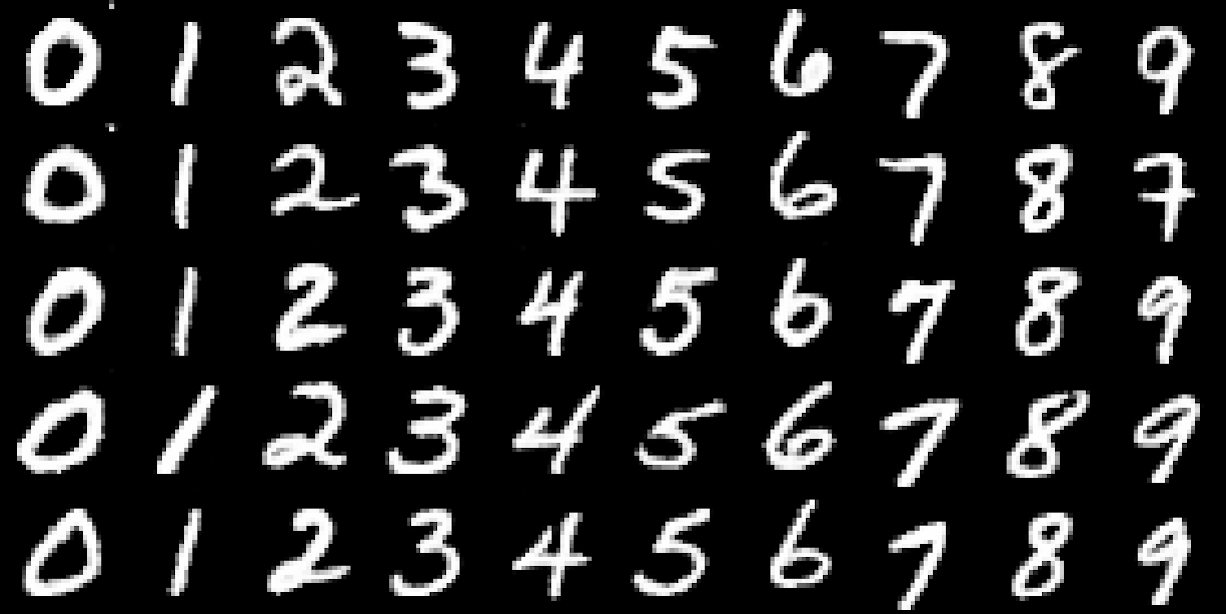
\includegraphics[width=.8\textwidth]{images/infogan_c1.png}
        \caption{Varying $\bm{c}_1 \in [0, 10]$}
    \end{subfigure}%
    \begin{subfigure}{.33\textwidth}
        \centering
        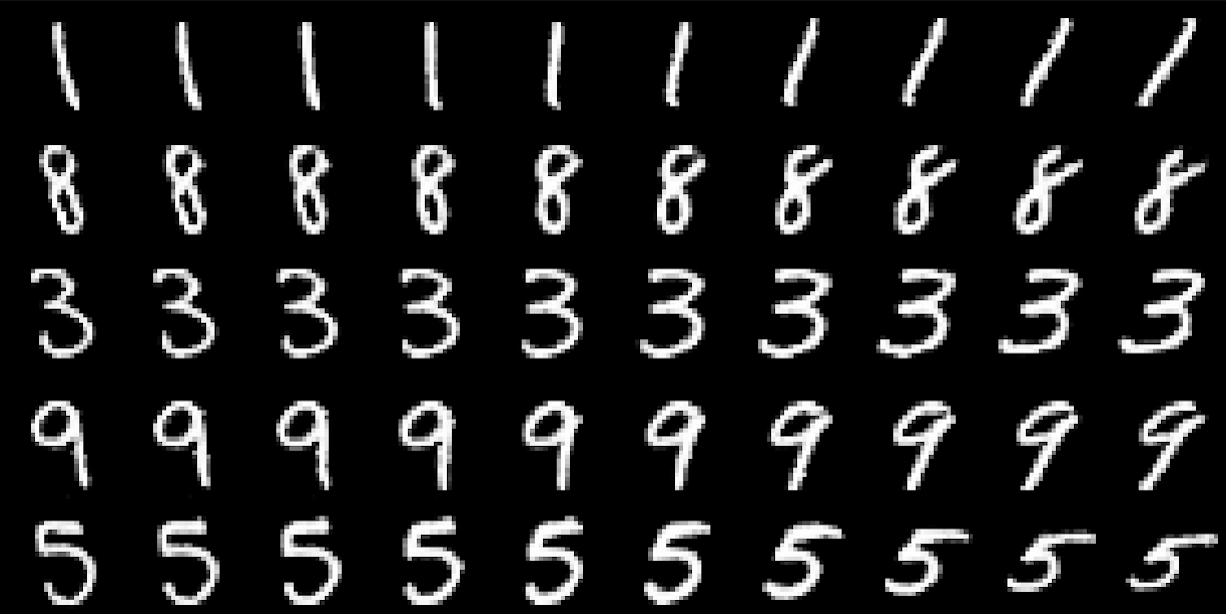
\includegraphics[width=.8\textwidth]{images/infogan_c2.png}
        \caption{Varying $\bm{c}_2 \in [-2, 2]$}
    \end{subfigure}
    \begin{subfigure}{.33\textwidth}
        \centering
        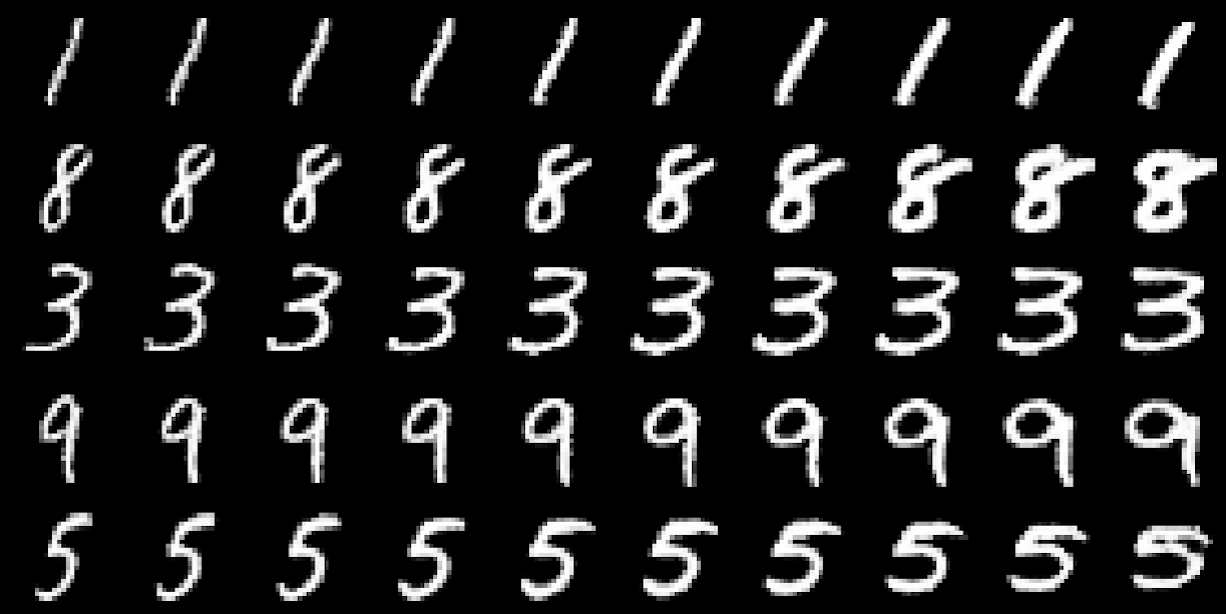
\includegraphics[width=.8\textwidth]{images/infogan_c3.png}
        \caption{Varying $\bm{c}_3 \in [-2, 2]$}
    \end{subfigure}
    \caption{Exploration of $\bm{c}$ on MNIST by systematically exploring either, $\bm{c}_1$, $\bm{c}_2$, or $\bm{c}_3$. Rows correspond to different noise values $\bm{z}$ but are equal for the three figures, columns correspond to different values for $\bm{c}_i$. $\bm{c}_1$ takes discrete values, $\bm{c}_2$ and $\bm{c}_3$ take continuous values. Taken from \citet{chen2016infogan}.}
    \label{fig:infogan}
\end{figure}

\say{To disentagle digit shape styles on MNIST}, \citet{chen2016infogan} choose $\bm{c}$ as three-element set $\bm{c} = (\bm{c}_1, \bm{c}_2, \bm{c}_3)$ with $\bm{c}_1$ drawn from a categorical distribution with ten categories (equal to the number of classes in MNIST) and event probability $p_i=0.1 \, \forall i \in [0, 10]$.
$\bm{c}_2$ and $\bm{c}_3$ are drawn from a uniform distribution over $[-1, 1]$.

Figure~\ref{fig:infogan} shows the representation disentaglement by varying the $\bm{c}_i$-values.
Noteworthy, InfoGAN seems to generalize as $\bm{c}_2$ and $\bm{c}_3$ varied between $[-2, 2]$ whereas these values took values in $[-1, 1]$ at training time.

\paragraph{\acl{LVAE}}

\aclp{LVAE}~\citep{sonderby2016ladder} address the problem of hierarchical learning in \acp{VAE}.
Hierarchical \acp{VAE} only use the first few layers to learn meaningful semantics of an input.
In case of \citet{sonderby2016ladder}, the first two layers are sufficient.
\citet{zhao2017learning} state that, given a sufficiently large encoder network in the first layer, the first layer learns all the semantics.
While this is not always true, they \say{demonstrate that this phenomen occurs in practive [\ldots]}.

\acp{LVAE} is a model designed to, instead of using just the first few layers, use all embedding layers to learn a representation.
They do this by passing information top-down in the inference network.
\begin{figure}
    \centering
    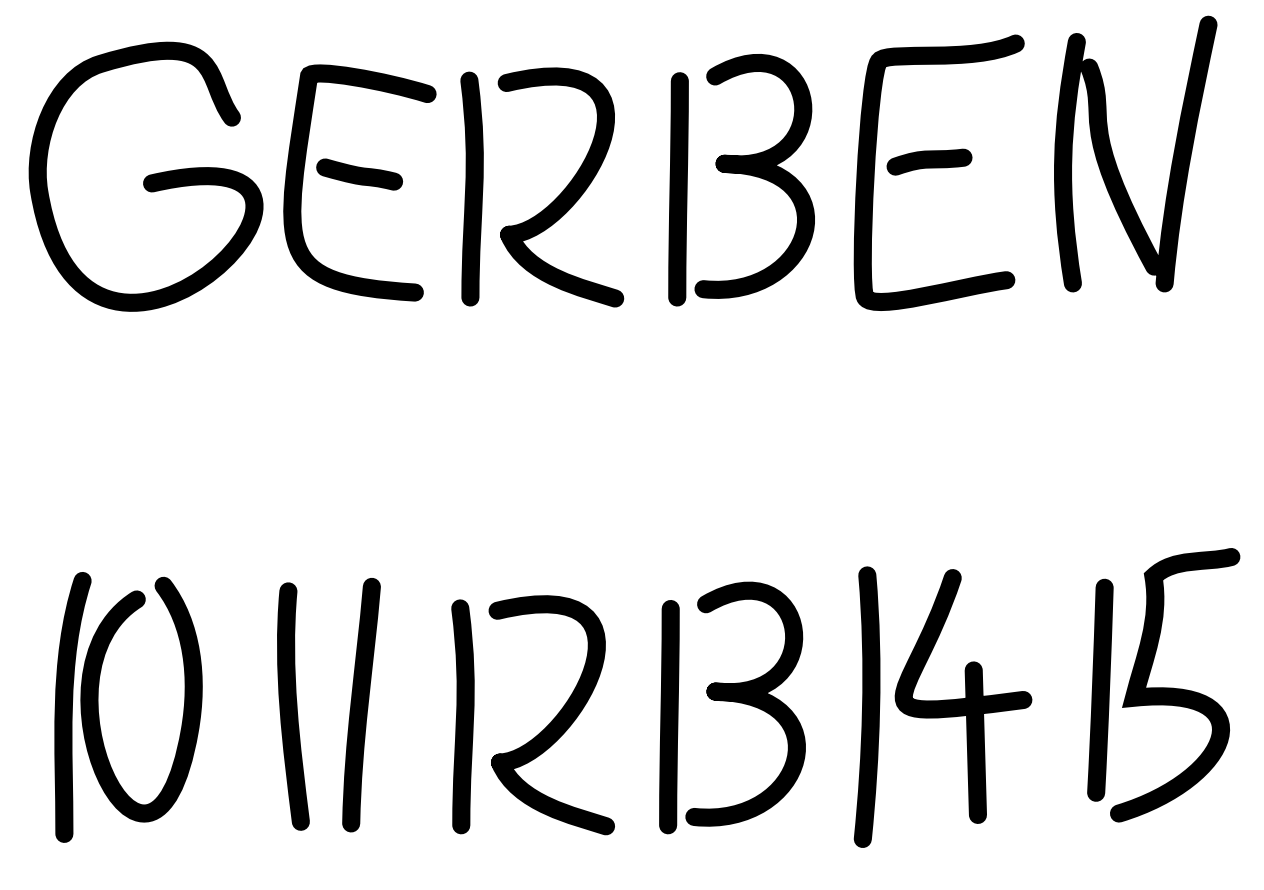
\includegraphics[width=0.2\textwidth]{images/gerben.png}
    \caption{Illustration of context-dependent semantic ambiguity. Taken from \citet[p. 61]{van2016auto}}
    \label{fig:gerben_ambiguity}
\end{figure}
Figure~\ref{fig:gerben_ambiguity} gives an intuition why passing information top-down can be advantegous.
Here, the two rows show two different alphanumeric strings.
Apparently, the first row shows a sequence of alphabetic characters (\say{GERBEN}) whereas the second row shows a sequence of numeric characters (\say{10 11 12 13 14 15}).
However, the \say{R} and the \say{B} in the first row are the exact same symbols as the \say{12} and the \say{13} in the second one.
A pure feed-forward systems would be unable to discriminate between the low-level features \textit{R} and \textit{13}.
Incorporating high-level features like \textit{alphabetic string} helps to improve the posterior low-level feature representation.
Furthermore, the additional top-down pass is more biologically plausible compared to a pure feedforward network (\textbf{REFERENCE}).

In fact, \acp{LVAE} model this top down pass by \textbf{BY WHAT? CONTINUE}
\begin{itemize}
    \item Explain LVAE detailed
    \item Dont forget the warm-up phase
    \item Also mention that batch normalization and warm-up alone help a lot in disentangling the feature learning
\end{itemize}

\paragraph{\acl{VLAE}}

\paragraph{Other stuff}
\begin{itemize}
    \item \citet{tschannen2018recent} give an overview over \say{recent advances in autoencoder-based representation learning}
\end{itemize}

\subsection{Visual Features in Neural Networks}\label{subsec:visual_features_in_neural_networks}
\begin{itemize}
    \item~\citet{krizhevsky2012imagenet} report Gabor wavelets in \acp{CNN} trained on image classification
    \item~\citet{palm2012prediction} found Gabor wavelets in vanilla autoencoders, trained on predicting the next image in a sequence, \citet{walker2016uncertain} did something similar for VAEs
    \item~\citet{eickenberg2017seeing} and \citet{wen2018neural} compare response of certain brain areas with layers in CNNs (also many more, a good list is in \citet{wen2018neural})
\end{itemize}

\subsection{Semantic Representations}\label{subsec:semantic-representations}

\subsubsection{Supervised Models}
\begin{itemize}
    \item \citet{khaligh2014deep} found evidence for that supervised models may explain \ac{IT} cortical representation
    \item \citet{cadieu2014deep} report more or less the same
\end{itemize}

\subsubsection{Unsupervised Models}
\begin{itemize}
    \item \citet{han2019variational} found no evidence for or against Gabor wavelets in \acp{VAE} due to too small kernel size, however they were able to predict fmri activity from the latent representation in a VAE
    \item \citet{khaligh2014deep} found evidence against the assumption that unsupervised models might explain \ac{IT} cortical representation, however not explicitly for \acp{VAE}
\end{itemize}